%Este trabalho está licenciado sob a Licença Creative Commons Atribuição-CompartilhaIgual 3.0 Não Adaptada. Para ver uma cópia desta licença, visite http://creativecommons.org/licenses/by-sa/3.0/ ou envie uma carta para Creative Commons, PO Box 1866, Mountain View, CA 94042, USA.

\documentclass[../livro.tex]{subfiles}  %%DM%%Escolher document class and options article, etc

% %%%%%%%%%%%%%%%%%%%%%%%%%%%%%%%%%%%%%%%%%%%%%%
% %%%%%%%%Pacotes básicos para MathEnvir%%%%%%%%
% %%%%%%%%%%%%%%%%%%%%%%%%%%%%%%%%%%%%%%%%%%%%%%

% \usepackage{amsmath}   %%AMS primary package (includes amstext, amsopn, amsbsy), provides various features for displayed equations and %%other mathematical constructs.
% %%%%OPTIONS FOR THE AMSMATH PACKAGE
% \usepackage{amscd}     %%Provides a CD environment for simple commutative diagrams (no support for diagonal arrows).
% \usepackage{amsxtra}   %%Provides certain odds and ends such as \fracwithdelims and \accentedsymbol, for compatibility with documents %%created using version 1.1.
% \usepackage{amsthm}    %%Enhanced version of \newtheorem command for defining theorem-like environments
% \usepackage{amssymb}   %%Provides an extended symbol collection (includes amsfonts). For example, \barwedge, \boxdot, \boxminus, %%\boxplus, \boxtimes, \Cap, \Cup (and many more), the arrow \leadsto, and some other symbols such as \Box and \Diamond.

% \usepackage{latexsym}  %%makes few additional characters available: \Box \Join \Box \Diamond \leadsto \sqsubset \sqsupset \lhd \unlhd %%\rhd \unrhd

% \usepackage[makeroom]{cancel}   % Cancelar termos em equações

% \usepackage{enumerate}

% %%%%%%%%%%%%%%%%%%%%%%%%%%%%%%%%%%%%%%%%%%%%%%
% %%%%%%%%Links -- Só funciona para .pdf%%%%%%%%
% %%%%%%%%%%%%%%%%%%%%%%%%%%%%%%%%%%%%%%%%%%%%%%

% %\usepackage{hyperref}  %% for references %%Options below
% %\hypersetup{colorlinks=true, linkcolor=blue, citecolor=blue, linktoc=page, pdftitle={Shadowing}, pdfauthor={D. Marcon}}

% %%%%%%%%%%%%%%%%%%%%%%%%%%%%%%%%%%%%%%%%%%%%%%
% %%%%%%Color, graphicx, margin (geometry)%%%%%%
% %%%%%%%%%%%%%%%%%%%%%%%%%%%%%%%%%%%%%%%%%%%%%%


% \usepackage[dvips]{graphicx}
% \usepackage{color}            %%Textcolor, color definitions, etc

% %\definecolor{light-blue}{rgb}{0.8,0.85,1}     %%Numbers between 0 and 1
% %\definecolor{mygrey}{gray}{0.75}              %%Numbers between 0 and 1

% \usepackage{verbatim}         %%Adds text from other files, comment environment

% \usepackage{xpatch}           %%Bold theorem titles
% \makeatletter
%    \xpatchcmd{\@thm}{\fontseries\mddefault\upshape}{}{}{} %same font as thm-header
% \makeatother

% \usepackage[margin=1in]{geometry}  %%Margins  %%Possible to use \newgeometry to modify small parts mid-document


% %fonte
% \usepackage{tgbonum}



% %%%%%%%%%%%%%%%%%%%%%%%%%%%%%%%%%%%%%%%%%%%%%
% %%%%%%%%%%%Para escrever português%%%%%%%%%%%
% %%%%%%%%%%%%%%%%%%%%%%%%%%%%%%%%%%%%%%%%%%%%%


% %\usepackage[utf8]{inputenc}  %%encoding
% %\usepackage[T1]{fontenc}     %%encoding

% \usepackage[portuguese]{babel}   %%Portuguese-specific commands



% %%%%%%%%%%%%%%%%%%%%%%%%%%%%%%%%%%%%%%%%%%%%%
% %%%%%%%%%%Theorem styles, numbering%%%%%%%%%%
% %%%%%%%%%%%%%%%%%%%%%%%%%%%%%%%%%%%%%%%%%%%%%


% \theoremstyle{plain}
% \newtheorem{theorem}{Teorema}              %%section, chapter, etc
% \newtheorem{proposition}[theorem]{Proposição}      %%everything below obeys theorem because: [theorem]
% \newtheorem{lemma}[theorem]{Lema}
% \newtheorem{corollary}[theorem]{Corolário}
% \newtheorem{maintheorem}{Teorema}                   %%number doesn't obey order
% \renewcommand{\themaintheorem}{\Alph{maintheorem}}
% \newtheorem{maincorollary}{Corolário}
% \newtheorem{conjecture}{Conjectura}
% \newtheorem*{claim}{Afirmação}

% \newtheorem*{desloct}{Segundo Teorema de Deslocamento -- Deslocamento em $t$}     %%Sem numeração e com o nome desejado

% \theoremstyle{definition}
% \newtheorem{remark}[theorem]{Observação}
% \newtheorem{example}[theorem]{Exemplo}
% \newtheorem{definition}[theorem]{Definição}
% \newtheorem{exercise}{Exercício}


% %%%%%%%%%%%%%%%%%%%%%%%%%%%%%%%%%%%%%%%%%%%%%
% %%%%%%%%%%%%%%%%New Commands%%%%%%%%%%%%%%%%%
% %%%%%%%%%%%%%%%%%%%%%%%%%%%%%%%%%%%%%%%%%%%%%

% \newcommand{\mb}[1]{\mathbb{#1}}
% \newcommand{\bC}{\mathbb{C}}
% \newcommand{\bE}{\mathbb{E}}
% \newcommand{\bK}{\mathbb{K}}
% \newcommand{\bN}{\mathbb{N}}
% \newcommand{\bP}{\mathbb{P}}
% \newcommand{\bQ}{\mathbb{Q}}
% \newcommand{\bR}{\mathbb{R}}
% \newcommand{\bS}{\mathbb{S}}
% \newcommand{\bT}{\mathbb{T}}
% \newcommand{\bZ}{\mathbb{Z}}

% \newcommand{\cB}{\mathcal{B}}
% \newcommand{\cE}{\mathcal{E}}
% \newcommand{\cF}{\mathcal{F}}
% \newcommand{\cH}{\mathcal{H}}
% \newcommand{\cL}{\mathcal{L}}
% \newcommand{\cM}{\mathcal{M}}
% \newcommand{\cO}{\mathcal{O}}
% \newcommand{\cP}{\mathcal{P}}
% \newcommand{\cQ}{\mathcal{Q}}
% \newcommand{\cR}{\mathcal{R}}
% \newcommand{\cS}{\mathcal{S}}

% \newcommand{\al} {\alpha}       \newcommand{\Al}{\Alpha}
% \newcommand{\be} {\beta}        \newcommand{\Be}{\Beta}
% \newcommand{\ga} {\gamma}       \newcommand{\Ga}{\Gamma}
% \newcommand{\de} {\delta}       \newcommand{\De}{\Delta}
% \newcommand{\ep} {\epsilon}
% \newcommand{\eps}{\varepsilon}
% \newcommand{\ze} {\zeta}
% \newcommand{\vte}{\vartheta}
% \newcommand{\iot}{\iota}
% \newcommand{\ka} {\kappa}
% \newcommand{\la} {\lambda}      \newcommand{\La}{\Lambda}
% \newcommand{\vpi}{\varpi}
% %\newcommand{\ro} {\rho}
% \newcommand{\vro}{\varrho}
% \newcommand{\si} {\sigma}       \newcommand{\Si}{\Sigma}
% \newcommand{\vsi}{\varsigma}
% \newcommand{\ups}{\upsilon}     \newcommand{\Up}{\Upsilon}
% \newcommand{\vphi}{\varphi}
% \newcommand{\om} {\omega}       \newcommand{\Om}{\Omega}

% \newcommand{\ang}{\operatorname{angle}}
% \newcommand{\closu}{\operatorname{clos}}
% \newcommand{\Col}{\operatorname{Col}}
% \newcommand{\const}{\operatorname{const}}
% \newcommand{\curl}{\operatorname{curl}}
% \newcommand{\dd}{\, \mathrm{d}}
% \newcommand{\diam}{\operatorname{diam}}
% \newcommand{\Dim}{\operatorname{dim}}
% \newcommand{\Div}{\operatorname{div}}
% \newcommand{\dist}{\operatorname{dist}}
% \newcommand{\grad}{\operatorname{grad}}
% \newcommand{\fr}{\partial}
% \newcommand{\graph}{\operatorname{graph}}
% \newcommand{\id}{\operatorname{Id}}
% \newcommand{\inter}{\operatorname{int}}
% \newcommand{\Leb}{\operatorname{Leb}}
% \newcommand{\length}{\operatorname{length}}
% \newcommand{\Lip}{\operatorname{Lip}}
% \newcommand{\Nul}{\operatorname{Nul}}
% \newcommand{\proj}{\operatorname{proj}}
% \newcommand{\res}{\operatornamewithlimits{Res}}
% \newcommand{\rot}{\operatorname{rot}}
% \newcommand{\sen}{\operatorname{sen}}
% \newcommand{\senh}{\operatorname{senh}}
% \newcommand{\Span}{\operatorname{Span}}
% \newcommand{\spec}{\operatorname{spec}}
% \newcommand{\supp}{\operatorname{supp}}
% \newcommand{\var}{\operatornamewithlimits{{var}}}
% \newcommand{\intd}{\operatornamewithlimits{{\iint}}}


% \everymath{\displaystyle}

% %%%%%%%%%%%%%%%%%%%%%%%%%%%%%%%%%%%%%%%%%%%%%
% %%%%%%%%%%%% INFO  DO  ARTIGO %%%%%%%%%%%%%%%
% %%%%%%%%%%%%%%%%%%%%%%%%%%%%%%%%%%%%%%%%%%%%%

% \title{Álgebra Linear -- Semana 12}
% %\author{}
% \date{\today}


%define o diretório principal
\providecommand{\dir}{..}

%%%%%%%%%%%%%%%%%%%%%%%%%%%%%%%%%%%%%%%%%%%%%
%%%%%%%%%%%%INICIO DO DOCUMENTO%%%%%%%%%%%%%%
%%%%%%%%%%%%%%%%%%%%%%%%%%%%%%%%%%%%%%%%%%%%%

\begin{document}

% \maketitle
% \tableofcontents

% \vspace{0.5cm}

\chapter{Semana 12}

\section{Projeção ortogonais sobre subespaços}

Na última semana, estudamos projeções ortogonais e vimos que a projeção ortogonal de $\vec{y}$ na direção de um vetor $\vec{w}$ pode ser calculada por
\begin{equation}
\proj_{\vec{w}} \vec{y} = \frac{\vec{y} \cdot \vec{w}}{\vec{w} \cdot \vec{w}} \ \vec{w}
\end{equation} Gostaríamos de endereçar agora a seguinte questão: como obter a projeção de um vetor $\vec{y} \in \bR^3$ sobre um plano $W$?

\begin{figure}[h!]
\begin{center}
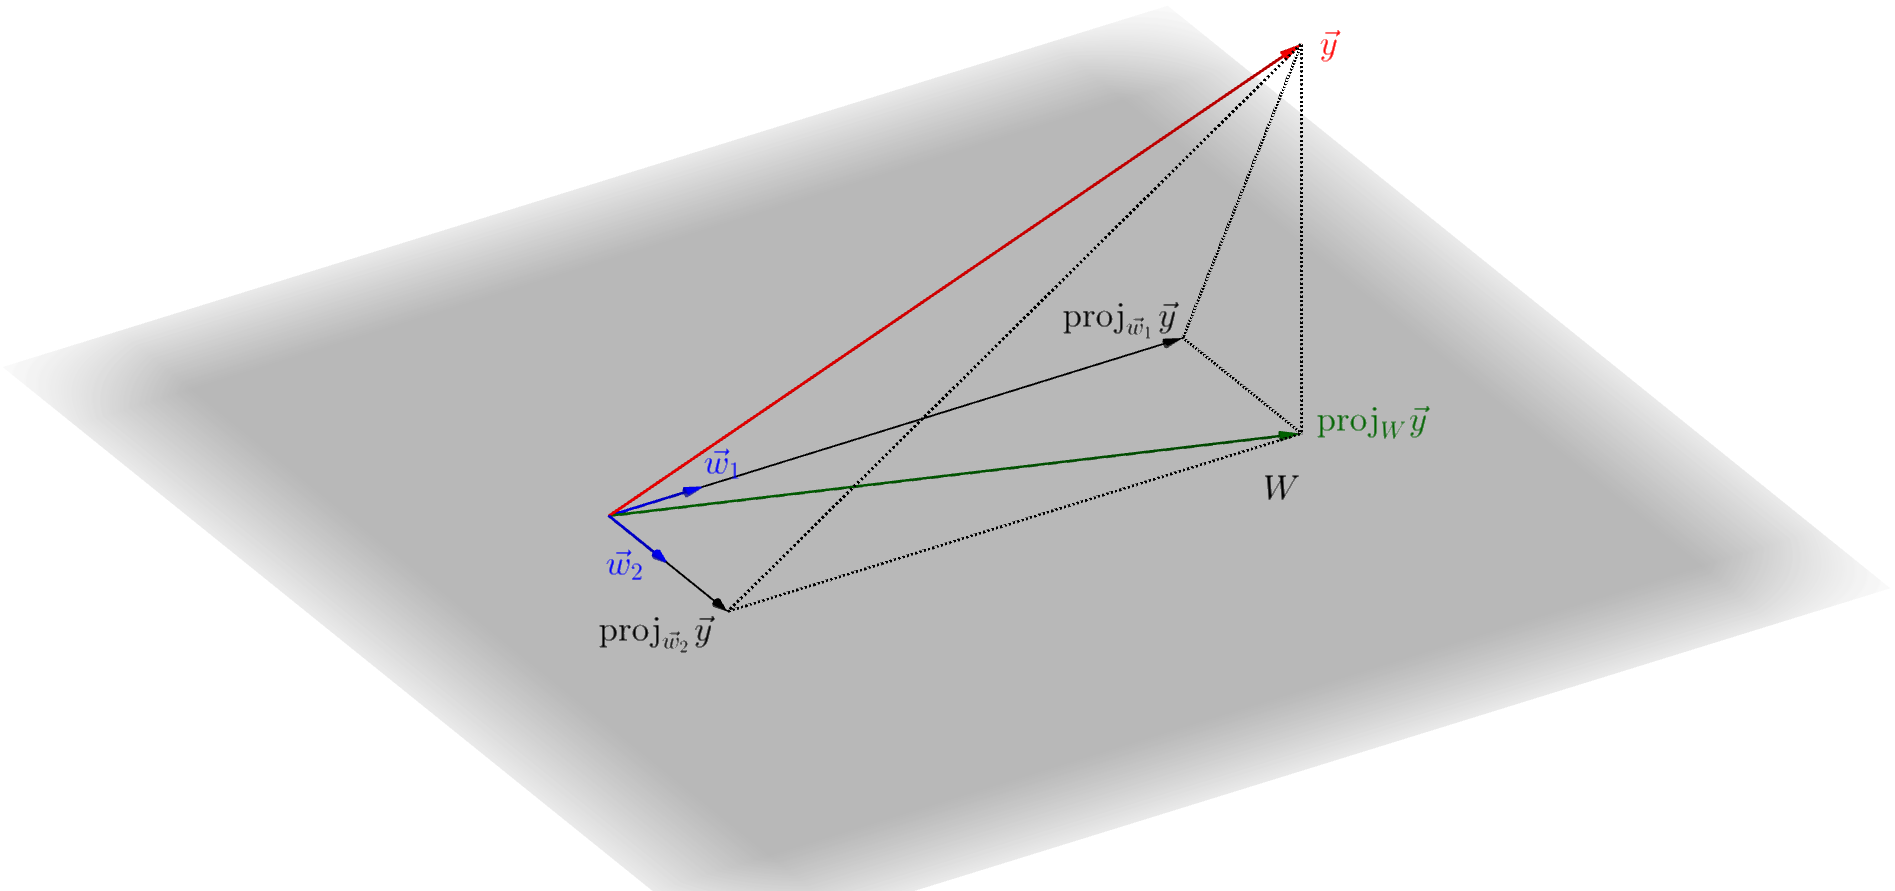
\includegraphics[width=0.6\linewidth]{\dir/Semana12/semana12-proj.png}
\end{center}
\end{figure}
\noindent Vamos trabalhar geométricamente: suponhamos que o plano
\begin{equation}
W = \Span \{\vec{w}_1, \vec{w}_2\}
\end{equation} e que os vetores $\vec{w}_1$ e $\vec{w}_2$ são ortogonais. Em outras palavras, $\{\vec{w}_1, \vec{w}_2\}$ é uma base ortogonal de $W$. Como veremos abaixo, o Processo de Gram-Schmidt fornece um algoritmo para obter uma base ortogonal de um espaço vetorial a partir de uma outra base qualquer e, logo, sempre é possível considerar uma base ortogonal.

A \textbf{projeção ortogonal sobre o subespaço $W$}, denotada por $\proj_W \vec{y}$, é definida como
\begin{equation}
\proj_W \vec{y} = \proj_{\vec{w}_1} \vec{y} + \proj_{\vec{w}_2} \vec{y} = \frac{\vec{y} \cdot \vec{w}_1}{\vec{w}_1 \cdot \vec{w}_1} \ \vec{w}_1 + \frac{\vec{y} \cdot \vec{w}_2}{\vec{w}_2 \cdot \vec{w}_2} \ \vec{w}_2.
\end{equation} Notamos que este vetor pertence a $W$, já que é uma combinação linear dos elementos de uma base de $W$. Mas mais fundamental é o fato de a projeção ser feita em uma direção ortogonal ao plano: devemos verificar que
\begin{equation}
\vec{y} - \proj_W \vec{y} \ \text{ é ortogonal a }  W.
\end{equation} Qualquer vetor de $W$ pode ser escrito como
\begin{equation}
\vec{w} = \frac{\vec{w} \cdot \vec{w}_1}{\vec{w}_1 \cdot \vec{w}_1} \ \vec{w}_1 + \frac{\vec{w} \cdot \vec{w}_2}{\vec{w}_2 \cdot \vec{w}_2} \ \vec{w}_2.
\end{equation}

\begin{exercise}
Utilize as propriedades do produto escalar e a ortogonalidade da base $\{\vec{w}_1, \vec{w}_2\}$ para verificar que
\begin{equation}
\vec{w} \cdot  \big( \vec{y} - \proj_W \vec{y} \big) = 0.
\end{equation}
\end{exercise}

\begin{example}
Vamos calcular a projeção do vetor
\begin{equation}
\vec{y} =
\begin{bmatrix}
 1\\1\\1
\end{bmatrix}
\end{equation} sobre o plano gerado pelos vetores
\begin{equation}
\vec{w}_1 =
\begin{bmatrix}
 0\\3\\-7
\end{bmatrix} \quad \text{e} \quad
\vec{w}_2 =
\begin{bmatrix}
 1\\0\\2
\end{bmatrix}.
\end{equation} Comlculamos
\begin{equation}
\begin{split}
\proj_W \vec{y} & = \frac{\vec{y} \cdot \vec{w}_1}{\vec{w}_1 \cdot \vec{w}_1} \ \vec{w}_1 + \frac{\vec{y} \cdot \vec{w}_2}{\vec{w}_2 \cdot \vec{w}_2} \ \vec{w}_2 = \frac{3-7}{9 + 49} \ \vec{w}_1 + \frac{1 + 2}{1+4} \ \vec{w}_2 \\
                & = -\frac{2}{29}
                \begin{bmatrix}
 0\\3\\-7
\end{bmatrix}
                + \frac{3}{5}
\begin{bmatrix}
 1\\0\\2
\end{bmatrix} =
\begin{bmatrix}
 3/5 \\ -6/29 \\ 244/145
\end{bmatrix}.
\end{split}
\end{equation}
\end{example}


Desenvolvemos acima o conceito de projeção ortogonal sobre um subespaço do espaço $\bR^3$ de dimensão três apenas pela conveniência da visualização geométrica. Na verdade, o conceito pode ser definido em qualquer dimensão.

Seja $W \subset \bR^n$ um subespaço vetorial de dimensão $k$ e $\{\vec{w}_1, \vec{w}_2, \dots, \vec{w}_k \}$ uma base ortogonal de $W$. Dado um vetor $\vec{y} \in \bR^n$ qualquer, definimos a \textbf{projeção ortogonal de $\vec{y}$ sobre $W$} como
\begin{equation}
\proj_W \vec{y}  = \frac{\vec{y} \cdot \vec{w}_1}{\vec{w}_1 \cdot \vec{w}_1} \ \vec{w}_1 + \frac{\vec{y} \cdot \vec{w}_2}{\vec{w}_2 \cdot \vec{w}_2} \ \vec{w}_2 + \cdots + \frac{\vec{y} \cdot \vec{w}_k}{\vec{w}_k \cdot \vec{w}_k} \ \vec{w}_k
\end{equation} Pode-se verificar, como no Exercício acima, que
\begin{equation}
\vec{w} \cdot  \big( \vec{y} - \proj_W \vec{y} \big) = 0, \ \text{para qualquer } \vec{w} \in W,
\end{equation} isto é, a projeção $\proj_W \vec{y}$ pertence a $W$ e $\vec{y} - \proj_W \vec{y}$ é ortogonal a todo elemento de $W$, assim como nossa intuição esperaria.


\begin{example}
Calcular a projeção do vetor
\begin{equation}
\vec{y} =
\begin{bmatrix}
1 \\ 0 \\ -1 \\ -3 \\ 2
\end{bmatrix}
\end{equation} sobre o espaço tridimensional gerado pelos vetores
\begin{equation}
\vec{w}_1 =
\begin{bmatrix}
 0\\4\\1 \\ 6 \\0
\end{bmatrix}, \quad
\vec{w}_2 =
\begin{bmatrix}
 1\\0\\2\\0\\-1
\end{bmatrix} \quad \text{e} \quad
\vec{w}_3 =
\begin{bmatrix}
 0\\0\\2\\4\\ 1
\end{bmatrix}.
\end{equation} Devemos calcular
\begin{equation}
\begin{split}
\proj_W \vec{y} & = \frac{\vec{y} \cdot \vec{w}_1}{\vec{w}_1 \cdot \vec{w}_1} \ \vec{w}_1 + \frac{\vec{y} \cdot \vec{w}_2}{\vec{w}_2 \cdot \vec{w}_2} \ \vec{w}_2 + \frac{\vec{y} \cdot \vec{w}_3}{\vec{w}_3 \cdot \vec{w}_3} \ \vec{w}_3\\
                & = \frac{ - 1 -18 }{ 16 + 1 + 36 } \ \vec{w}_1 + \frac{ 1 - 2 - 2 }{ 1 + 4 + 1 } \ \vec{w}_2 + \frac{ -2-12+2 }{ 4 + 16 + 1 } \ \vec{w}_3 \\
                & = -\frac{19}{53} \begin{bmatrix}
 0\\4\\1 \\ 6 \\0
\end{bmatrix} - \frac{1}{2} \begin{bmatrix}
 1\\0\\2\\0\\-1
\end{bmatrix} - \frac{12}{21} \begin{bmatrix}
 0\\0\\2\\4\\ 1
\end{bmatrix} =
\begin{bmatrix}
 -1/2 \\ -76/53 \\ -2784/1113 \\ -4938/1113 \\ -1/12
\end{bmatrix}.
\end{split}
\end{equation}Confira estas contas com uma calculadora (os coeficientes dos vetores nem sempre são bonitinhos!)
\end{example}



\section{Distância a subespaços e a melhor aproximação}


A projeção ortogonal pode ser utilizada para calcular distâncias entre o pontos e subespaços.

\begin{figure}[h!]
\begin{center}
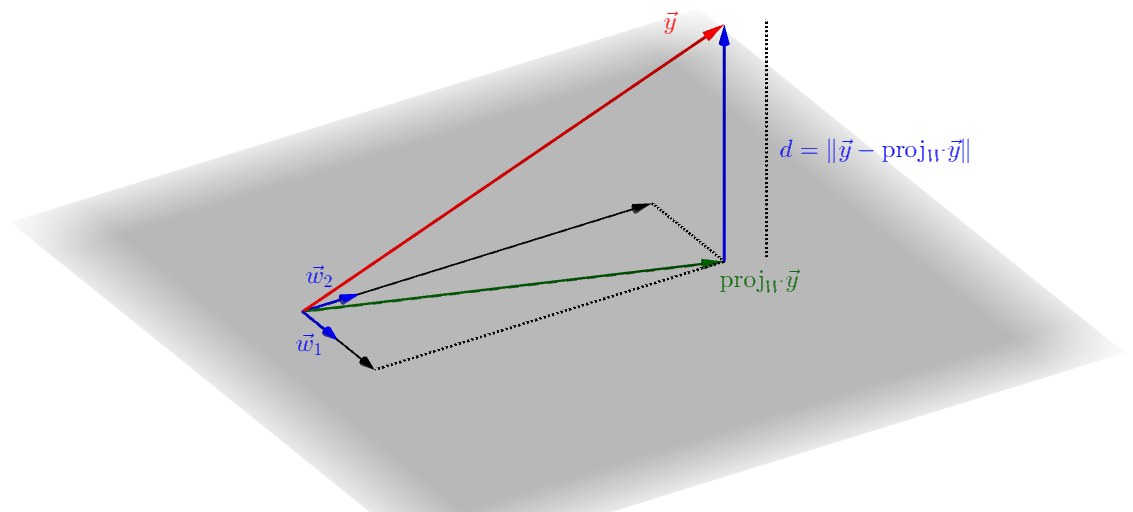
\includegraphics[width=0.6\linewidth]{\dir/Semana12/semana12-dist.png}
\end{center}
\end{figure}

\noindent Dado um ponto $P = (x_1, x_2, \dots, x_n)$, formamos o vetor
\begin{equation}
\vec{y} =
\begin{bmatrix}
x_1 \\ x_2 \\ \vdots \\ x_n
\end{bmatrix}
\end{equation} cujas componentes são as coordenadas de $P$. Como vimos na seção anterior, o vetor $\vec{y} - \proj_{W} \vec{y}$ é ortogonal ao subespaço $W$. Sendo a distância de $P$ até $W$ denotada por $\dist (P,W)$ e definida como a menor distância entre $P$ e elementos de $W$, temos que
\begin{equation}
\dist (P,W) = \|\vec{y} - \proj_{W} \vec{y}\|.
\end{equation}


\begin{proof}[Justificativa desta afirmação]
Dado qualquer outro vetor $\vec{w} \in W$, o Teorema de Pitágoras implica que (ver figura)
\begin{equation}
\| \vec{y} - \vec{w} \|^2 = \| \vec{w} - \proj_{W} \vec{y}\|^2 + \| \vec{y} - \proj_{W} \vec{y}\|^2 > \| \vec{y} - \proj_{W} \vec{y}\|^2.
\end{equation} Em outras palavras, $\|\vec{y} - \proj_{W} \vec{y}\|$ é de fato a menor distância entre $P$ e elementos de $W$.
\begin{figure}[h!]
\begin{center}
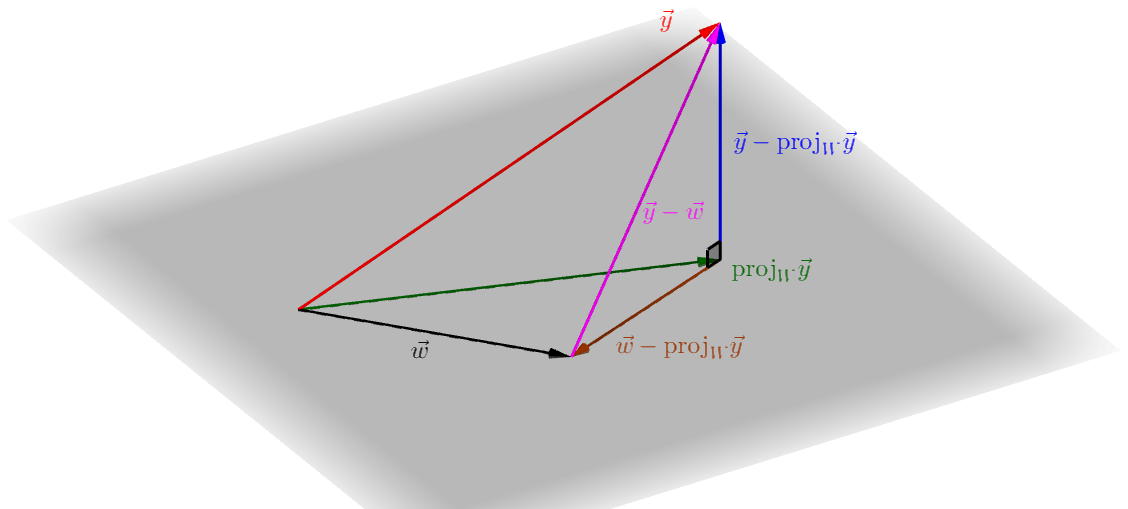
\includegraphics[width=0.6\linewidth]{\dir/Semana12/semana12-dist-justif.png}
\end{center}
\end{figure}
\end{proof}


\begin{example}
Calcular a distância do ponto $P = (1,2,-1,0,7)$ até o plano $W = \Span\{\vec{u}, \vec{v}\}$ (contido em $\bR^5$) gerado pelos vetores
\begin{equation}
\vec{u} =
\begin{bmatrix}
1 \\ 0 \\ 2 \\ 0 \\ 5
\end{bmatrix} \ \text{e} \ \
\vec{v} = \begin{bmatrix}
1 \\ -1 \\ 2 \\ 0 \\ 3
\end{bmatrix}.
\end{equation} Para isto, consideramos o vetor
\begin{equation}
\vec{y} = \begin{bmatrix}
1 \\ 2 \\ -1 \\ 0 \\ 7
\end{bmatrix}
\end{equation}e vamos calcular $\|\vec{y} - \proj_W \vec{y}\|$:
\begin{equation}
\begin{split}
\vec{y} - \proj_W \vec{y} & = \vec{y} - \frac{\vec{y} \cdot \vec{u}}{\vec{u} \cdot \vec{u}} \ \vec{u} - \frac{\vec{y} \cdot \vec{v}}{\vec{v} \cdot \vec{v}} \ \vec{v}  =
\begin{bmatrix}
1 \\ 2 \\ -1 \\ 0 \\ 7
\end{bmatrix} - \frac{34}{30}
\begin{bmatrix}
1 \\ 0 \\ 2 \\ 0 \\ 5
\end{bmatrix} - \frac{18}{15}
\begin{bmatrix}
1 \\ -1 \\ 2 \\ 0 \\ 3
\end{bmatrix} \\
   & = \begin{bmatrix}
1 \\ 2 \\ -1 \\ 0 \\ 7
\end{bmatrix} - \frac{17}{15}
\begin{bmatrix}
1 \\ 0 \\ 2 \\ 0 \\ 5
\end{bmatrix} - \frac{18}{15}
\begin{bmatrix}
1 \\ -1 \\ 2 \\ 0 \\ 3
\end{bmatrix} =
\begin{bmatrix}
-4/3 \\ 16/5 \\ -17/3 \\ 0 \\ -34/15
\end{bmatrix}
\end{split}
\end{equation} Desta forma, a distância de $P$ a $W$ é
\begin{equation}
\begin{split}
\dist (P,W) & = \|\vec{y} - \proj_{W} \vec{y}\| = \sqrt{\frac{16}{9} + \frac{256}{25} + \frac{289}{9} + \frac{1156}{225}} = \sqrt{\frac{ 16\cdot 25 + 256\cdot 9 + 289 \cdot 25 + 1156}{225}} \\
           & = \frac{ \sqrt{11085} }{15} \simeq 7,02.
\end{split}
\end{equation}
\end{example}




\section{O Processo de ortogonalização de Gram--Schmidt}

O \textbf{Processo de Gram--Schmidt} é um algoritmo para obter uma base ortogonal (ou ortonormal) a partir de uma base qualquer. De maneira mais geral, o método permite transformar um conjunto de vetores linearmente independentes em um conjunto ortogonal que gera o mesmo espaço vetorial. 

Vamos começar com um exemplo.

\begin{example}
Consideramos os vetores
\begin{equation}
\vec{v}_1 =
\begin{bmatrix}
1 \\ 0 \\ 1
\end{bmatrix}, \quad
\vec{v}_2 =
\begin{bmatrix}
1 \\ 1 \\ 0
\end{bmatrix} \quad \text{e} \quad
\vec{v}_3 =
\begin{bmatrix}
0 \\ 1 \\ 1
\end{bmatrix}.
\end{equation} O espaço gerado por $\{\vec{v}_1, \vec{v}_2, \vec{v}_3 \}$ é todo o espaço $\bR^3$, já que temos três vetores  linearmente independentes em um espaço de dimensão três.

O processo consiste em fixar qualquer um dos vetores como o primeiro dos vetores do conjunto que virá a ser ortogonal. Por exemplo, fixamos
\begin{equation}
\vec{u}_1 = \vec{v}_1 =
\begin{bmatrix}
1 \\ 0 \\ 1
\end{bmatrix}.
\end{equation} Em seguida, já vimos que, ao fazer a projeção de $\vec{v}_2$ sobre $\vec{v}_1$, o vetor
\begin{equation}
\vec{v}_2 - \proj_{\vec{v}_1} \vec{v}_2
\end{equation} é ortogonal a $\vec{v}_1$, como ilustra a figura.
\begin{figure}[h!]
\begin{center}
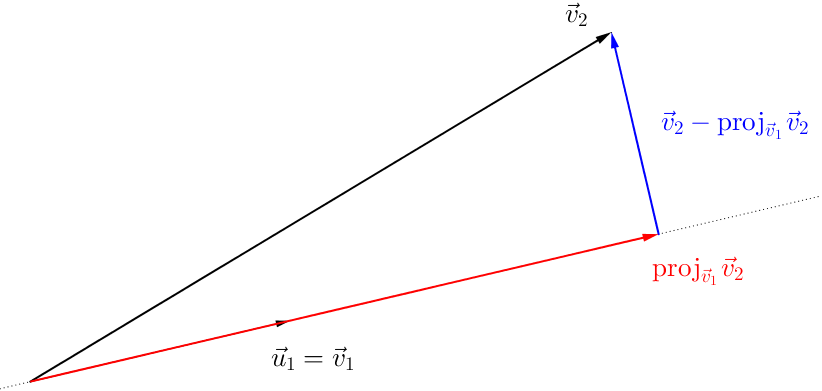
\includegraphics[width=0.6\linewidth]{\dir/Semana12/semana12-gram1.png}
\end{center}
\end{figure}

\noindent Assim sendo, definimos o segundo vetor do nosso conjunto que será ortogonal como o vetor
\begin{equation}
\vec{u}_2 = \vec{v}_2 - \proj_{\vec{u}_1} \vec{v}_2 = \vec{v}_2 - \frac{\vec{v}_2 \cdot \vec{u}_1}{\vec{u}_1 \cdot \vec{u}_1} \, \vec{u}_1 =
\begin{bmatrix}
1 \\ 1 \\ 0
\end{bmatrix}
- \frac{1}{2}
\begin{bmatrix}
1 \\ 0 \\ 1
\end{bmatrix} =
\begin{bmatrix}
1/2 \\ 1 \\ -1/2
\end{bmatrix} = \frac{1}{2}
\begin{bmatrix}
1 \\ 2 \\ -1
\end{bmatrix}.
\end{equation} Temos que $\vec{u}_1$ e $\vec{u}_2$ são ortogonais e que estão no mesmo plano, de modo que também temos
\begin{equation}
\Span \{ \vec{u}_1, \vec{u}_2 \} = \Span \{ \vec{v}_1, \vec{v}_2 \}.
\end{equation} Vamos escrever momentariamente $W = \Span \{ \vec{u}_1, \vec{u}_2 \}$.

No próximo passo do processo, o terceiro vetor pode ser obtido como
\begin{equation}
\vec{u}_3 = \vec{v}_3 - \proj_{W} \vec{v}_3,
\end{equation} pois, desta forma, $\vec{u}_3$ é ortogonal a todos os vetores de $W$; em particular, é ortogonal a ambos $\vec{u}_1$ e $\vec{u}_2$. Além disso, como $\vec{u}_1$ e $\vec{u}_2$ já são vetores ortogonais, podemos calcular a projeção sobre $W$ como de costume:
\begin{equation}
\vec{u}_3 = \vec{v}_3 - \proj_{W} \vec{v}_3 = \vec{v}_3 - \frac{\vec{v}_3 \cdot \vec{u}_1}{\vec{u}_1 \cdot \vec{u}_1} \, \vec{u}_1 - \frac{\vec{v}_3 \cdot \vec{u}_2}{\vec{u}_2 \cdot \vec{u}_2} \, \vec{u}_2.
\end{equation}
\begin{figure}[h!]
\begin{center}
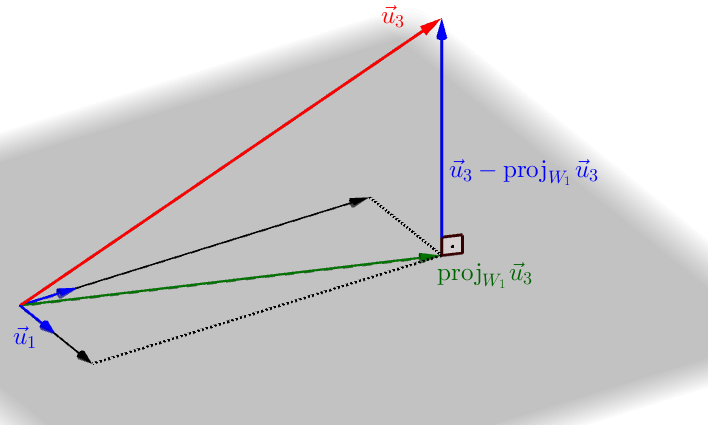
\includegraphics[width=0.6\linewidth]{\dir/Semana12/semana12-gram2.png}
\end{center}
\end{figure}

\noindent Calculando, temos (observe como dois fatores $1/2$ cancelam no último termo)
\begin{equation}
\vec{u}_3 =
\begin{bmatrix}
0 \\ 1 \\ 1
\end{bmatrix}  - \frac{1}{2}
\begin{bmatrix}
1 \\ 0 \\ 1
\end{bmatrix} - \frac{2 - 1}{1 + 4 +1}
\begin{bmatrix}
1 \\ 2 \\ -1
\end{bmatrix} =
\begin{bmatrix}
0 \\ 1 \\ 1
\end{bmatrix}  - \frac{1}{2}
\begin{bmatrix}
1 \\ 0 \\ 1
\end{bmatrix} - \frac{1}{6}
\begin{bmatrix}
1 \\ 2 \\ -1
\end{bmatrix} =
\begin{bmatrix}
-2/3 \\ 2/3 \\ 2/3
\end{bmatrix} = \frac{2}{3}
\begin{bmatrix}
-1 \\ 1 \\ 1
\end{bmatrix}
\end{equation} Concluimos assim que o conjunto
\begin{equation}
\{ \vec{u}_1, \vec{u}_2, \vec{u}_3 \} = \left\{
\begin{bmatrix}
1 \\ 0 \\ 1
\end{bmatrix},
\begin{bmatrix}
1/2 \\ 1 \\ -1/2
\end{bmatrix},
\begin{bmatrix}
-2/3 \\ 2/3 \\ 2/3
\end{bmatrix}  \right\}
\end{equation} é ortogonal e gera o mesmo espaço que $\{ \vec{v}_1, \vec{v}_2, \vec{v}_3 \}$.

Na realidade, se tivéssemos considerado múltiplos dos vetores acima, não perderíamos a propriedade de ortogonalidade, e temos
\begin{equation}
\Span \{ \vec{u}_1, \vec{u}_2, \vec{u}_3 \} =
\Span \left\{
\begin{bmatrix}
1 \\ 0 \\ 1
\end{bmatrix},
\begin{bmatrix}
1 \\ 2 \\ -1
\end{bmatrix},
\begin{bmatrix}
-1 \\ 1 \\ 1
\end{bmatrix}
\right\}.
\end{equation} ``Colocar em evidência'' os fatores comuns desta forma e ``desconsiderá-los'' pode facilitar as contas em alguns casos.

Observamos também que, fazendo a normalização dos vetores, podemos obter uma base ortonormal:
\begin{equation}
\left\{
  \begin{array}{ll}
   \|\vec{u}\| = \sqrt{1 + 0 + 1} = \sqrt{2} \\
   \|\vec{v}\| = \sqrt{1 + 4 + 1} = \sqrt{6} \\
   \|\vec{w}\| = \sqrt{1 + 1 + 1} = \sqrt{3} \\
  \end{array}
\right.
\end{equation} e assim,
\begin{equation}
\frac{\vec{u}_1}{\|\vec{u}_1\|} = \frac{1}{\sqrt{3}}
\begin{bmatrix}
1 \\ 0 \\ 1
\end{bmatrix} =
\begin{bmatrix}
1/\sqrt{2} \\ 0 \\ 1/\sqrt{2}
\end{bmatrix}, \
\frac{\vec{u}_2}{\|\vec{u}_2\|} = \frac{1}{\sqrt{6}}
\begin{bmatrix}
1 \\ 2 \\ -1
\end{bmatrix} =
\begin{bmatrix}
1/\sqrt{6} \\ 2/\sqrt{6} \\ -1/\sqrt{6}
\end{bmatrix} \ \text{e }
\frac{\vec{u}_3}{\|\vec{u}_3\|} = \frac{1}{\sqrt{3}}
\begin{bmatrix}
-1 \\ 1 \\ 1
\end{bmatrix} =
\begin{bmatrix}
-1/\sqrt{3} \\ 1/\sqrt{3} \\ 1/\sqrt{3}
\end{bmatrix}
\end{equation} forma um conjunto ortonormal que gera o mesmo espaço vetorial que $\{ \vec{v}_1, \vec{v}_2, \vec{v}_3 \}. \ \lhd$
\end{example}



Em seguida, mostramos como funciona o processo de maneira geral (um bom entendimento do exemplo acima deve deixar claro o porquê deste processo funcionar): sejam $k$ vetores linearmente independentes $\vec{v}_1, \vec{v}_2, \cdots, \vec{v}_k$ pertencentes ao espaço $n$-dimensional $\bR^n$. Vamos denotar
\begin{equation}
W = \Span \{\vec{v}_1, \vec{v}_2, \cdots, \vec{v}_k\}
\end{equation} e construir uma base ortogonal (e em seguida ortonormal) para $W$. Começamos com
\begin{equation}
\boxed{\vec{u}_1 = \vec{v}_1}
\end{equation} e definimos
\begin{equation}
\boxed{\vec{u}_2 = \vec{v}_2 - \proj_{\vec{u}_1} \vec{v}_2 = \vec{v}_2 - \frac{\vec{v}_2 \cdot \vec{u}_1}{\vec{u}_1 \cdot \vec{u}_1} \, \vec{u}_1.}
\end{equation} Temos que $\vec{u}_1$ e $\vec{u}_2$ são ortogonais e que estão no mesmo plano, de modo que também temos
\begin{equation}
\Span \{ \vec{u}_1, \vec{u}_2 \} = \Span \{ \vec{v}_1, \vec{v}_2 \} = W_2 \ \leftrightsquigarrow \text{ notação.}
\end{equation} Em seguida, definimos
\begin{equation}
\boxed{\vec{u}_3 = \vec{v}_3 - \proj_{W_2} \vec{v}_3 = \vec{v}_3 - \frac{\vec{v}_3 \cdot \vec{u}_1}{\vec{u}_1 \cdot \vec{u}_1} \, \vec{u}_1 - \frac{\vec{v}_3 \cdot \vec{u}_2}{\vec{u}_2 \cdot \vec{u}_2} \, \vec{u}_2.}
\end{equation} Temos que $\vec{u}_1, \vec{u}_2, \vec{u}_3$ ortogonais e
\begin{equation}
\Span \{ \vec{u}_1, \vec{u}_2, \vec{u}_3 \} = \Span \{ \vec{v}_1, \vec{v}_2, \vec{v}_3 \} = W_3 \ \leftrightsquigarrow \text{ notação.}
\end{equation} Em seguida
\begin{equation}
\boxed{\vec{u}_4 = \vec{v}_4 - \proj_{W_3} \vec{v}_4 = \vec{v}_4 - \frac{\vec{v}_4 \cdot \vec{u}_1}{\vec{u}_1 \cdot \vec{u}_1} \, \vec{u}_1 - \frac{\vec{v}_4 \cdot \vec{u}_2}{\vec{u}_2 \cdot \vec{u}_2} \, \vec{u}_2 - \frac{\vec{v}_4 \cdot \vec{u}_3}{\vec{u}_3 \cdot \vec{u}_3} \, \vec{u}_3.}
\end{equation} Temos que $\vec{u}_1, \vec{u}_2, \vec{u}_3, \vec{u}_4$ ortogonais e
\begin{equation}
\Span \{ \vec{u}_1, \vec{u}_2, \vec{u}_3, \vec{u}_4 \} = \Span \{ \vec{v}_1, \vec{v}_2, \vec{v}_3, \vec{u}_4 \} = W_4 \ \leftrightsquigarrow \text{ notação.}
\end{equation} E assim seguimos fazendo as contas até chegar ao último vetor: sendo
\begin{equation}
\Span \{ \vec{u}_1, \vec{u}_2, \cdots, \vec{u}_{k-1} \} = \Span \{ \vec{v}_1, \vec{v}_2, \cdots, \vec{v}_{k-1} \} = W_{k-1} \ \leftrightsquigarrow \text{ notação,}
\end{equation} escrevemos
\begin{equation}
\boxed{\vec{u}_k = \vec{v}_k - \proj_{W_{k-1}} \vec{v}_k = \vec{v}_k - \frac{\vec{v}_k \cdot \vec{u}_1}{\vec{u}_1 \cdot \vec{u}_1} \, \vec{u}_1 - \frac{\vec{v}_k \cdot \vec{u}_2}{\vec{u}_2 \cdot \vec{u}_2} \, \vec{u}_2 - \cdots - \frac{\vec{v}_k \cdot \vec{u}_{k-1}}{\vec{u}_{k-1} \cdot \vec{u}_{k-1}} \, \vec{u}_{k-1}.}
\end{equation} Temos que $\{\vec{u}_1, \vec{u}_2, \dots, \vec{u}_k\}$ é um conjunto ortogonal e
\begin{equation}
\Span \{ \vec{u}_1, \vec{u}_2, \dots, \vec{u}_k \} = \Span \{ \vec{v}_1, \vec{v}_2, \dots, \vec{u}_k \} = W \ \leftrightsquigarrow \text{ que é o espaço inicial, }
\end{equation} como queríamos.

Este é a parte mais ``pesada'' do método. Por exemplo, se agora quiséssemos uma base ortonormal para $W$, basta considerar o conjunto
\begin{equation}
\left\{ \frac{\vec{u}_1}{\|\vec{u}_1\|}, \frac{\vec{u}_2}{\|\vec{u}_2\|}, \dots, \frac{\vec{u}_k}{\|\vec{u}_k\|} \right\},
\end{equation} que continua sendo ortogonal, mas agora formado por vetores unitários.




\begin{example}[Retirado de Wikipedia.org]
Vamos obter uma base ortonormal para o espaço coluna $\Col A$ da matriz
\begin{equation}
A =
\begin{bmatrix}
12 & -51 & 4 \\
6 & 167 & -68 \\
-4 & 24 & -41
\end{bmatrix}.
\end{equation} Lembrando que $\Col A$ é o espaço gerado pelas colunas de $A$, vamos aplicar o processo de Gram--Schmidt para os vetores
\begin{equation}
\vec{v}_1 =
\begin{bmatrix}
12 \\
6 \\
-4
\end{bmatrix},
\vec{v}_2 =
\begin{bmatrix}
 -51  \\
 167  \\
 24
\end{bmatrix}, \vec{v}_3 =
\begin{bmatrix}
  4 \\
 -68 \\
 -41
\end{bmatrix}.
\end{equation} O Processo começa como:
\begin{equation}
\begin{split}
\vec{u}_1 & = \vec{v}_1 =
\begin{bmatrix}
12 \\
6 \\
-4
\end{bmatrix}, \\
\vec{u}_2 &  = \vec{v}_2 - \frac{\vec{v}_2 \cdot \vec{u}_1}{\vec{u}_1 \cdot \vec{u}_1} \, \vec{u}_1 =
\begin{bmatrix}
 -51  \\
 167  \\
 24
\end{bmatrix} - \frac{-612 +1002 - 96}{144 + 36 + 16}
\begin{bmatrix}
12 \\
6 \\
-4
\end{bmatrix} =
\begin{bmatrix}
 -51  \\
 167  \\
 24
\end{bmatrix} - \frac{296}{196}
\begin{bmatrix}
12 \\
6 \\
-4
\end{bmatrix} =
\begin{bmatrix}
 -69  \\
 158  \\
 30
\end{bmatrix}
\end{split}
\end{equation} Em seguida (conferir estas contas com o auxílio de uma calculadora)
\begin{equation}
\begin{split}
\vec{u}_3 & = \vec{v}_3 - \frac{\vec{v}_3 \cdot \vec{u}_1}{\vec{u}_1 \cdot \vec{u}_1} \, \vec{u}_1 - \frac{\vec{v}_3 \cdot \vec{u}_2}{\vec{u}_2 \cdot \vec{u}_2} \, \vec{u}_2 = \begin{bmatrix}
  4 \\
 -68 \\
 -41
\end{bmatrix} - \frac{48-408 + 164}{196}
\begin{bmatrix}
12 \\
6 \\
-4
\end{bmatrix} - \frac{-276 - 10744 - 1230}{4761 + 24694 + 900}
\begin{bmatrix}
 -69  \\
 158  \\
 30
\end{bmatrix} \\
   & = \begin{bmatrix}
  4 \\
 -68 \\
 -41
\end{bmatrix} + \cancel{\frac{196}{196}}
\begin{bmatrix}
12 \\
6 \\
-4
\end{bmatrix} + \frac{12250}{30355}
\begin{bmatrix}
 -69  \\
 158  \\
 30
\end{bmatrix} = \begin{bmatrix}
 -58/5  \\
 6/5  \\
 -33
\end{bmatrix}.
\end{split}
\end{equation} Para obter uma base ortonormal para o espaço coluna, vamos ainda considerar
\begin{equation}
\frac{\vec{u}_1}{\|\vec{u}_1\|}, \frac{\vec{u}_2}{\|\vec{u}_2\|}, \frac{\vec{u}_3}{\|\vec{u}_3\|}.
\end{equation} Calculamos
\begin{equation}
\left\{
  \begin{array}{ll}
   \|\vec{u}_1\| = \sqrt{196} = 14 \\
   \|\vec{u}_2\| = \sqrt{30625} = 175 \\
   \|\vec{u}_3\| = \frac{\sqrt{30625}}{5} = 35
  \end{array}
\right.
\end{equation} Portanto, uma base ortonormal para $\Col A$ é
\begin{equation}
\vec{n}_1 = \frac{\vec{u}_1}{\|\vec{u}_1\|} =
\begin{bmatrix}
 6/7  \\
 3/7  \\
 -2/7
\end{bmatrix}, \quad
\vec{n}_2 = \frac{\vec{u}_2}{\|\vec{u}_2\|} =
\begin{bmatrix}
 -69/175  \\
 158/175  \\
 6/35
\end{bmatrix} \quad \text{e} \quad
\vec{n}_3 = \frac{\vec{u}_3}{\|\vec{u}_3\|} =
\begin{bmatrix}
 -58/175  \\
 6/175  \\
 -33/35
\end{bmatrix}. \lhd
\end{equation}
\end{example}


\section{Fatoração QR e matrizes ortogonais}


O método de Gram-Schmidt nos permite fatorar uma matriz $A$ cujas colunas são LI em um produto \begin{equation}A=QR,\end{equation} onde Q é uma matriz cujas colunas formam um conjunto ortonormal e $R$ é uma matriz triangular superior. Tal fatoração é muito importante do ponto de vista computacional, como veremos em breve, quando usarmos a fatoração QR como uma alternativa  para resolução de sistemas lineareas por mínimos quadrados. Também é a base de um eficiente método numérico para encontrar autovalores de uma matriz quadrada.

Matrizes cujas colunas formam um conjunto ortonormal são muito úteis e por isso recebem um nome especial:são chamadas de matrizes ortogonais. Aqui cabe uma observação relevante: este é um exemplo de uma situação onde a terminologia clássica está longe de ser satisfatória: matrizes  cujas colunas formam um conjunto {\it ortonormal} são chamadas de matrizes {\it ortogonais}.   

\medskip

Faremos agora uma exposição da fatoração QR usando uma matriz inicial $A$ que tem 3 colunas, observando que a construção abaixo é facilmente generalizada para uma matriz de qualquer dimensão (desde que tenha colunas LI).

Dada uma matriz $A=[\vec{v}_1 \vec{v}_2 \vec{v}_3]$ cujas colunas são LI e são denotadas por $\vec{v}_1$, $\vec{v}_2$, e $\vec{v}_3$, 
o processo de Gram-Schmidt começa com a construção de uma base ortogonal formada pelos vetores
$\vec{u}_1$, $\vec{u}_2$, e $\vec{u}_3$,
para o espaço-coluna da matriz $A$. Para isso, definimos

\begin{equation}
\begin{cases}
\vec{u}_1 = \vec{v}_1 \\ 
\vec{u}_2 = \vec{v}_2 - \proj_{\vec{u}_1} \vec{v}_2 \\
\vec{u}_3 = \vec{v}_3 - \proj_{\vec{u}_1,\vec{u}_2} \vec{v}_3
\end{cases}
\end{equation}
Portanto existem coeficientes $b_1$, $c_1$ e $c_2$ tais que 
\begin{equation}
\begin{cases}
\vec{u}_1 = \vec{v}_1 \\ 
\vec{u}_2 = \vec{v}_2 - b_1 \vec{u}_1 \\
\vec{u}_3 = \vec{v}_3 - c_1 \vec{u}_1 - c_2 \vec{u}_2
\end{cases}
\end{equation}

Em um segundo momento, cada um dos três vetores $\vec{u}_1$, $\vec{u}_2$, e $\vec{u}_3$ é normalizado, ou seja, dividimos cada um deles pelo seu comprimento. Assim, $\vec{u}_1$, $\vec{u}_2$, e $\vec{u}_3$ formam uma base ortonormal para o espaço coluna de $A$, e  existem coeficientes $\alpha_1$, $\beta_1$, $\beta_2$, $\gamma_1$, $\gamma_2$ e $\gamma_3$ tais que 
\begin{equation}
\begin{cases}
\vec{u}_1 = \alpha_1\vec{v}_1 \\ 
\vec{u}_2 = \beta_2 \vec{v}_2 - \beta_1 \vec{u}_1 \\
\vec{u}_3 = \gamma_3 \vec{v}_3 - \gamma_1 \vec{u}_1 - \gamma_2 \vec{u}_2
\end{cases}
\end{equation}
Se colocarmos as colunas da matriz $A$ em função dos vetores da base ortonormal que acaba de ser obtida, temos 
\begin{equation}
\begin{cases}
\vec{v}_1 = \alpha_1^{-1}\vec{u}_1 \\ 
\vec{v}_2 = \beta_2^{-1} \vec{u}_2 + \beta_2^{-1}\beta_1 \vec{u}_1 \\
\vec{v}_3 = \gamma_3^{-1} \vec{u}_3 + \gamma_3^{-1}\gamma_1 \vec{u}_1 + \gamma_3^{-1}\gamma_2 \vec{u}_2
\end{cases}
\end{equation}
ou trocando a ordem das parcelas no lado direito,
\begin{equation}
\begin{cases}
\vec{v}_1 = \alpha_1^{-1}\vec{u}_1 \\ 
\vec{v}_2 =  \beta_2^{-1}\beta_1 \vec{u}_1 + \beta_2^{-1} \vec{u}_2 \\
\vec{v}_3 =   \gamma_3^{-1}\gamma_1 \vec{u}_1 + \gamma_3^{-1}\gamma_2 \vec{u}_2 + \gamma_3^{-1} \vec{u}_3
\end{cases}
\end{equation}
Assim, ao definirmos a matriz $Q=[\vec{u}_1 \vec{u}_2  \vec{u}_3] $, obtemos \begin{equation}A=QR\end{equation}
onde 
\begin{equation}
R =
\begin{bmatrix}
\alpha_1^{-1}  & \beta_2^{-1}\beta_1  & \gamma_3^{-1}\gamma_1 \\
0 & \beta_2^{-1} & \gamma_3^{-1}\gamma_2 \\
0 & 0 & \gamma_3^{-1}
\end{bmatrix}
\end{equation}
visto que cada coluna do produto $QR$, é definido como a combinação linear das colunas da matriz $Q$ com pesos dados pela respectiva coluna da matriz $R$.

Note ainda que $R$ é invertível, visto que sua diagonal principal contém apenas termos não-nulos.

A construção acima é facilmente generalizada para matrizes quaisquer e nos permite enunciar o seguinte fato
(lembre que uma matriz ortogonal é uma matriz cujas colunas formam um conjunto ortonormal):

\begin{theorem}
Qualquer matriz $A$ cujas colunas são linearmente independentes pode ser fatorada na forma $A=QR$, onde $Q$ é uma matriz ortogonal 
e $R$ é uma matriz triangular superior invertível. Ainda, o espaço coluna das matrizes $A$ e $Q$ é o mesmo, ou seja, as colunas de $Q$ formam uma base ortonormal para o subespaço gerado pelas colunas de $A$.
\end{theorem} 

Note que a fatoração QR está para o processo de Gram-Schmidt assim como a fatoração LU está para o método de  linha-redução a forma escada!  %\footnote{Preciso escrever sobre a fatoração LU. Acho que seria interessante também mostrar que matrizes ortogonais preservam comprimento e ângulo.}

Bem, vimos que a matriz $Q$ tem como colunas a base ortonormal gerada pelo processo de Gram-Schmidt. E como podemos calcular a matriz $R$ no caso geral ? 

Usando o seguinte fato surpreendente: 

\begin{theorem}
uma matriz ortogonal é sempre invertível e sua inversa é dada pela sua transposta, ou seja $Q^{-1}= Q^T$.
\end{theorem}


A prova deste teorema é simples:
 
\begin{equation}
Q^T Q =
\begin{bmatrix}
 \text{--- }\  \vec{u}_1 \, \text{ ---} \\
 \text{--- }\  \vec{u}_2 \, \text{ ---} \\
 \text{--- }\  \vec{u}_3 \, \text{ ---}
\end{bmatrix}
\begin{bmatrix}
 | & | & | \\
\vec{u}_1 & \vec{u}_2 & \vec{u}_3 \\
 | & | & |
\end{bmatrix} =
\begin{bmatrix}
 \vec{u}_1 \cdot \vec{u}_1 & \vec{u}_1 \cdot \vec{u}_2 & \vec{u}_1 \cdot \vec{u}_2 \\
 \vec{u}_2 \cdot \vec{u}_1 & \vec{u}_2 \cdot \vec{u}_2 & \vec{u}_2 \cdot \vec{u}_3 \\
 \vec{u}_3 \cdot \vec{u}_1 & \vec{u}_3 \cdot \vec{u}_2 & \vec{u}_3 \cdot \vec{u}_3
\end{bmatrix} =
\begin{bmatrix}
1 & 0 & 0 \\
0 & 1 & 0 \\
0 & 0 & 1
\end{bmatrix} = I.
\end{equation}

Assim, se $A=QR$, basta multiplicar ambos os lados desta equação por $Q^T$ pela esquerda para obtermos:

\begin{equation}Q^T A = Q^T Q R  \Longrightarrow R= Q^T A.\end{equation}






\vspace{0.3cm}



No último exemplo da seção anterior, obtemos através do método de Gram-Schmidt uma base ortonormal para $\Col A$
onde 
\begin{equation}
A =
\begin{bmatrix}
12 & -51 & 4 \\
6 & 167 & -68 \\
-4 & 24 & -41
\end{bmatrix}.
\end{equation}
Vamos definir a matriz $Q$ como a matriz formada pelos vetores desta base ortonormal:
\begin{equation}
Q =
\begin{bmatrix}
6/7 & -69/175 & -58/175 \\
3/7 & 158/175 & 6/175   \\
-2/7& 6/35   &-33/35
\end{bmatrix}
\end{equation} 

%tem, portanto, suas colunas ortonormais. 
%É possível verificar que ao fazermos $Q^T A$ obtemos uma matriz triangular $R$. Podemos escrever
Vimos que $R=Q^T A$ e portanto
\begin{equation}
R = Q^T A =
\begin{bmatrix}
6/7 & 3/7 & -2/7 \\
-69/175 & 158/175 & 6/35   \\
-58/175& 6/175   &-33/35
\end{bmatrix}
\begin{bmatrix}
12 & -51 & 4 \\
6 & 167 & -68 \\
-4 & 24 & -41
\end{bmatrix} =
\begin{bmatrix}
14&21&-14\\
0&175&-70\\
0&0&35
\end{bmatrix} .
\end{equation} 
Finalmente podemos escrever
\begin{equation}
A =
\begin{bmatrix}
12 & -51 & 4 \\
6 & 167 & -68 \\
-4 & 24 & -41
\end{bmatrix} =
\begin{bmatrix}
6/7 & -69/175 & -58/175 \\
3/7 & 158/175 & 6/175   \\
-2/7& 6/35   &-33/35
\end{bmatrix}
\begin{bmatrix}
14&21&-14\\
0&175&-70\\
0&0&35
\end{bmatrix} = QR. \ \lhd
\end{equation}


\section{Matrizes Ortogonais preservam comprimento e ângulo}

Vamos aproveitar para falar um pouco mais sobre matrizes ortogonais. Um bom exemplo de matriz ortogonal $2\times 2$ é dada pela matriz de rotação, ou seja, pela matriz

\begin{equation}
Q =
\begin{bmatrix}
\cos (\theta) & -\sin (\theta) \\
\sin (\theta) & \cos (\theta) 
\end{bmatrix} ,\end{equation}
onde $0 \leq \theta \leq 2 \pi$.
Podemos ver que esta matriz define uma transformação linear no plano que rotaciona vetores em um ângulo $\theta$ no sentido anti-horário.
Assim, tal transformação preserva comprimento e ângulo entre vetores.
Estas propriedades não são particulares da matriz de rotação: todas as matrizes ortogonais se comportam da mesma forma. O teorema a seguir traz estas informações e mais algumas.

\begin{theorem}
	Seja $Q=[\vec{u}_1,...,\vec{u}_n]$ uma matriz ortogonal $n \times n$. Então, para quaisquer vetores $\vec{v}$ e $\vec{w}$ em $\mathbb{R}^n$ temos
	\begin{enumerate}
		\item[i.] $Q\vec{v} \cdot Q\vec{w} = \vec{v} \cdot  \vec{w}$
		\item[ii.]  $\| Q\vec{v} \| = \| \vec{v} \|$
		\item[iii.]  o ângulo entre $Q\vec{v}$ e $Q\vec{w}$ é igual ao  ângulo entre $\vec{v}$ e $\vec{w}$
		\end{enumerate}
\end{theorem}

A prova do primeiro item é consequência direta da linearidade do produto interno e da hipótese das colunas formarem uma base ortonormal: se $\vec{v} = (\alpha_1,..., \alpha_n)$ e $\vec{w} = (\beta_1, ..., \beta_n)$,  então

\begin{equation}Q\vec{v} \cdot Q\vec{w} = \left( \sum_{i=1}^n \alpha_i \vec{u}_i \right) \cdot \left(   \sum_{j=1}^n \beta_j \vec{u}_j \right) =  \sum_{i=1}^n \sum_{j=1}^n \alpha_i \beta_j \;\vec{u}_i \cdot \vec{u}_j\end{equation} 
devido a linearidade do produto interno (ou seja a propriedade distributiva aplicada tanto na primeira quanto na segunda componente do produto interno). Agora, lembrando que $\vec{u}_i \cdot \vec{u}_j=0$ se $i \neq j$, a ultima expressão iguala-se a 
\begin{equation} \sum_{i=1}^n \alpha_i \beta_i \; \vec{u}_i \cdot \vec{u}_i.\end{equation}
Finalmente, lembrando que cada coluna $\vec{u}_i$ de $Q$ tem comprimento unitário, concluimos que
\begin{equation}Q\vec{v} \cdot Q\vec{w} = \sum_{i=1}^n \alpha_i \beta_i = \vec{v} \cdot \vec{w}.\end{equation}
 
 
 Os próximos dois itens seguem diretamente do primeiro item, visto que 
\begin{equation}\| Q \vec{v} \| = \sqrt{Q\vec{v} \cdot Q\vec{v}} = \sqrt{\vec{v} \cdot \vec{v}} =  \| \vec{v} \| \end{equation} 
e 
o ângulo entre $Qv$ e $Qw$ é definido como 
\begin{equation}
\arccos\left(\frac{Qv \cdot Qw	}{\|Qv\| \|Qw\|} \right)
=\arccos\left(\frac{v \cdot w	}{\|v\| \|w\|} \right),\end{equation} 
que por definição é o ângulo  entre $v$ e $w$. 
Assim finalizamos a prova do teorema. 
 
 \medskip
 
 
 Um outro exemplo de matriz ortogonal é dado pelas matrizes de reflexão. Um caso particular é dado pela reflexão em torno do eixo horizontal: 
 
 \begin{equation}
 Q =
 \begin{bmatrix}
 1 & 0 \\
 0 & -1
 \end{bmatrix} .\end{equation}


\end{document} 





Finalizamos esta seção enunciando um teorema cujo primeiro item já foi provado e cujo segundo item é consequencia direta do primeiro e do fato de que $\det(AB)=\det(A) \det (B)$:  PS NAO VALE A PENA PRECISA DE ALGO MAIS...

\begin{theorem}
	Seja $Q=[\vec{u}_1,...,\vec{u}_n]$ uma matriz ortogonal. Temos
	\begin{enumerate}
		\item[i.] $Q^{-1}=Q^T$
		\item[ii.] $\det(Q)=1$ ou $\det(Q)=-1$.
	\end{enumerate}
\end{theorem}